\documentclass[a4j, twocolumn, 10pt]{jsarticle}

\usepackage[dvipdfmx]{graphicx, color}
\usepackage[top=20truemm,bottom=20truemm,left=15truemm,right=15truemm]{geometry}
\usepackage{wrapfig}

\definecolor{High}{cmyk}{0.00, 0.96, 0.39, 0.00}
\definecolor{Low}{cmyk}{0.80, 0.20, 0.00, 0.00}

% \renewcommand{\kanjifamilydefault}{\gtdefault} % 日本語書体をゴシック体に
\renewcommand{\familydefault}{\sfdefault} % 欧文書体をHelveticaに

\title{とてもめずらしい疾患を持ったX歳の男児の一例}
\author{高橋 亨平\thanks{国立病院機構 岡山医療センター 小児科 \texttt{kcrt@kcrt.net}}}
\date{\today}

\begin{document}

\maketitle
\section{症例:X歳男児}
\subsection*{主訴}
なんらかの訴え
\subsection*{現病歴}
今まで検診で異常を指摘されたことはない。X月になんらかの訴えで受診し治療目的に当院入院となった。

\subsection*{既往歴}
\begin{itemize}
\setlength{\itemsep}{0cm}
\item X歳:不思議な疾患
\end{itemize}
\subsection*{内服}
なし
\subsection*{入院時身体所見}
\noindent
身長: XXXcm (+X.XSD), 体重: XX.Xkg($\pm$X.XSD)\\
体温: XX.X$^{\circ}{\rm C}$, SpO$_{2}$: XX.X\% \\
心拍数: XX拍/分, 血圧: XXX/XX[mmHg]\\
呼吸音: 清 ラ音なし、心音: 整 雑音なし\\
腹部: 平坦、軟、圧痛なし 腸蠕動音聴取\\
眼瞼・顔面・四肢いずれも浮腫を認めない
\subsection*{入院時検査所見}
\subsubsection*{CBC}
\begin{tabular}[thb]{rrl|rrl}
WBC & XXXX & /$\mu L$ & RBC & X.XX & $\times 10^{6}/\mu L$ \\
 Seg. & XX.X & \% & Hb & XX.X & $g/dL$ \\
 Eos. & XX.X & \% & Ht & XX.X & $\%$ \\
 Bas. & XX.X & \% & Plt & XX.X & 万/mL \\
 Mon. & XX.X & \% & & \\
 Lym. & XX.X & \% & & \\
\end{tabular}
\subsubsection*{生化学}
\subsubsection*{凝固}
\subsubsection*{尿検査}

\subsection*{入院後の経過}
\begin{figure*}[!htb]
	\centering
	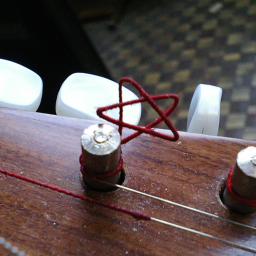
\includegraphics[width=3cm, bb=0 0 184 184]{/Users/kcrt/etc/kcrt.png}
	\caption{不思議な経過図}
\end{figure*}
入院の後でいろいろな検査をしていろいろなことがわかった。
\subsection*{検査結果}
いろいろな検査結果です。

\subsubsection*{特殊な検査}
\begin{itemize}
\item AAAA
\item BBBB
\item CCCC
\end{itemize}
\setlength\intextsep{0pt}

\subsection*{その後の経過}
いろいろあって退院することができた。

\section{考察}
世の中わからないことばかりである。

\end{document}
